\documentclass[12pt,fleqn]{article}\usepackage{../common}
\begin{document}
Ders 15

Bu onemli bir ders, ana konumuz yansitma / projeksiyon (projection). Mesela
$b$ vektorunu alip $a$ uzerine olan ``yansimasini'' hesaplamak. 

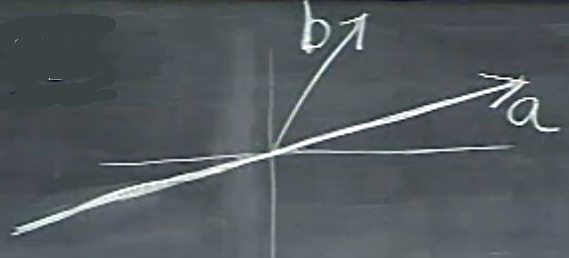
\includegraphics[height=2cm]{15_1.png}




\end{document}
